\documentclass[fleqn]{article}
\usepackage{tikz,tcolorbox}
\usepackage{array} % For customizing tables
\usepackage{booktabs} % For better horizontal lines
\usepackage[a4paper, paperwidth=25cm, paperheight=25.5cm, left=2cm, right=2cm, top=2cm, bottom=2cm]{geometry}
\usepackage{multicol}
\usepackage{amsmath}
\usepackage{pgfplots}

\usepackage{tkz-tab}

\usepackage{enumitem}

\pgfplotsset{compat=1.18}
\usepackage{makecell}
\usetikzlibrary{patterns}
\definecolor{mygreen}{HTML}{14C877}
\definecolor{orangePlot}{HTML}{EA6E12}
\definecolor{purplePlot}{HTML}{4C12EA}
\definecolor{blueArea}{HTML}{10D9EE}
\definecolor{redPlot}{HTML}{ED014A}
\definecolor{myblue}{HTML}{338AC7}
\definecolor{p}{HTML}{D813E7}
\definecolor{y}{HTML}{F5F806}
\usepackage{amssymb}
\setlength{\parindent}{0pt}
\setcellgapes{3pt}  % Adjust padding as needed
\makegapedcells
\tcbuselibrary{skins, breakable, theorems}
\usepackage{algorithm}
\usepackage{algpseudocode}
\usepackage{xcolor}
\setlength{\mathindent}{8cm}
\renewcommand{\thealgorithm}{}
\usepackage{mathtools}
\newtcolorbox{prettyBox}[2]{
  enhanced,
  colback=white!90!#2,   % Background color based on the second parameter (color)
  colframe=#2!60!black,  % Frame color based on the second parameter (color)
  coltitle=white,        % Title color (white)
  fonttitle=\bfseries\Large,
  title=#1,              % Title from the first parameter
  boxrule=1mm,
  arc=0.5mm,
  drop shadow=#2!35!gray, % Drop shadow color based on the second parameter (color)
}

\usepackage{listings}

\definecolor{keywordcolor}{RGB}{0, 128, 255}   % Blue for keywords
\definecolor{directivecolor}{RGB}{255, 0, 255} % Magenta for Flex directives
\definecolor{stringcolor}{RGB}{0, 180, 0}      % Green for strings
\definecolor{commentcolor}{RGB}{128, 128, 128} % Gray for comments
\definecolor{operatorcolor}{RGB}{255, 102, 0} 




\lstdefinelanguage{Flex}{
    morekeywords={\%\%, int,char,while,if,else,return, \%\{, \%\}, \%option, \%x, \%s, \%pointer, \%ar, \%top, \%yymore, \%input, \%output, \%yywrap, \%yynewline},
    morestring=[b]{"},
    sensitive=true,
    alsoletter={\%, \}, \{},
}
% Define cstyle
\lstdefinestyle{cstyle}{
    language=Flex,
    basicstyle=\ttfamily\small,
    keywordstyle=\color{blue},
    stringstyle=\color{green!50!black},
    numbers=left,
    numberstyle=\tiny\color{gray},
    stepnumber=1,
    numbersep=5pt,
    backgroundcolor=\color{white},
    frame=single,
    frameround=tttt,
    rulecolor=\color{black},
    breaklines=true,
    breakatwhitespace=true,
    tabsize=4,
    showspaces=false,
    showstringspaces=false,
    showtabs=false,
    captionpos=b,
    escapeinside={(*}{*)}
}

\lstdefinestyle{simple}{
    basicstyle=\ttfamily,       % Use a monospaced font
    numbers=left,               % Enable line numbers on the left
    numberstyle=\tiny\color{gray}, % Make line numbers smaller and gray
    stepnumber=1,               % Number every line
    firstnumber=1,              % Start numbering from line 1
    frame=single,               % Start numbering from line 1
}
\begin{document}
\renewcommand{\arrayrulewidth}{0.75mm} % Set line thickness
\setlength{\tabcolsep}{12pt} % Set horizontal padding
\renewcommand{\arraystretch}{1.5} % Set vertical padding (1.0 is default)

\begin{center}
    \Huge{\textbf{\underline{Devoir Maison Numero 1}}}
\end{center}

\vspace{1cm}

\begin{center}
    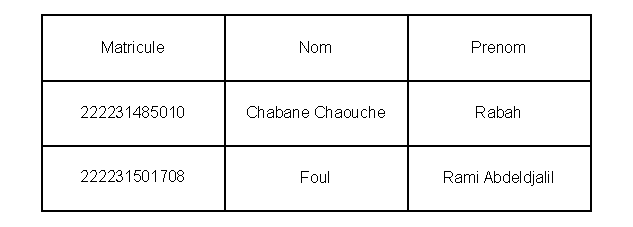
\includegraphics[width=0.9\textwidth]{Parts/bi.drawio.pdf}
\end{center}

\newpage

\section{Langage}
\subsection{Entités Lexicales Du Langage}
\begin{prettyBox}{Entités Lexicales}{mygreen}
\begin{itemize}
    \item \textbf{Identifiants} : les noms des variables , et fonctions.
    \item \textbf{Mots Clés} :
        \begin{itemize}
            \item \textbf{Type Prédéfinis} : 'Entier', 'Reel'.
            \item \textbf{Délimiteurs De Bloc} : 'Begin', 'end', 'Body', 'Declaration', 'MainProgram'.
        \end{itemize}
    \item \textbf{Constantes} :
         \begin{itemize}
             \item \textbf{Constante Entière}
             \item \textbf{Constante Chaine De Caractères}
         \end{itemize}
    \item \textbf{Séparateurs} :
        \begin{itemize}
            \item \textbf{Opération Arithmétique} : '/', '+', '-', '*'.
            \item \textbf{Parenthèses} : '(', ')'.
            \item \textbf{Accolades} : '\{' , '\}'.
            \item \textbf{Affectation} : ':='.
            \item \textbf{Deux Points} : ':'.
            \item \textbf{Virgule et Point-Virgule} : ',', ';'.
        \end{itemize}
\end{itemize}
\end{prettyBox}

\vspace{1cm}

\subsection{Commentaires}
\begin{prettyBox}{Commentaires}{mygreen}
    \begin{itemize}
        \item \textbf{Commentaire Simple} : commentaire écrit en 
            une ligne commençant par '\#\#'.
        \item \textbf{Commentaire Multi-ligne} : commentaire qui peut
            être écrit sur plusieurs lignes, commence par '\{ \texttt{--}' et finit par '\texttt{--} \}'.
    \end{itemize}
\end{prettyBox}



\newpage
\section{Implementation En Flex}

\begin{center}
    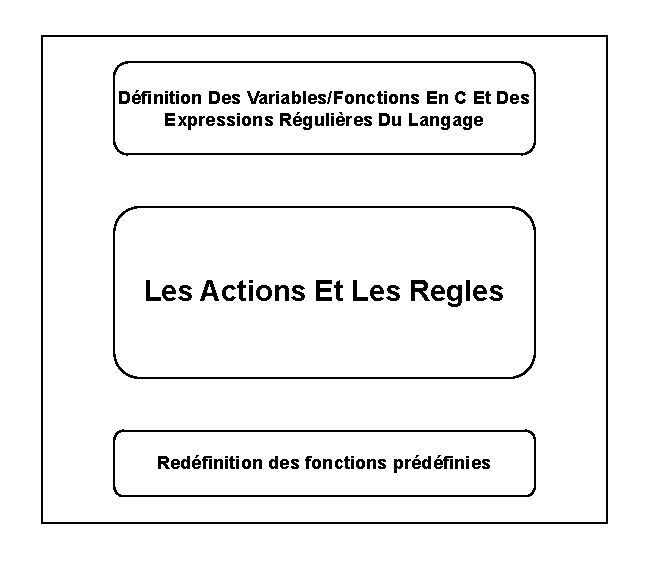
\includegraphics[width=0.9\textwidth]{Parts/flex.drawio.pdf}
\end{center}

\newpage
\subsection{Définition Des Variables/Fonctions Des Expressions Régulières}

\subsubsection{Variables Et Fonctions}
\begin{prettyBox}{Variables}{mygreen}
\begin{itemize}
    \item \textbf{Variable Entière : }\texttt{nb\_line} qu'on va incrémenter 
pour chaque saut de ligne \texttt{\textbackslash n} initialisé a 1.
    \item \textbf{Bibliothèque : }\texttt{<stdio.h>} pour afficher des messages avec 
\texttt{printf}.
    \item \textbf{Fonction : }\texttt{nb\_line\_comment} calcule le nombre de saut de ligne 
        contenue dans un commentaire.
\end{itemize}
\end{prettyBox}

\vspace{0.5cm}
\textbf{\underline{Code}}

\vspace{0.25cm}
\lstinputlisting[style=cstyle,firstline=1,lastline=17,basicstyle=\footnotesize\ttfamily]{Parts/solution.l}

\vspace{0.5cm}

\subsubsection{Expressions Régulières}
\begin{prettyBox}{Expressions Régulières}{mygreen}
    \begin{itemize}
        \item \textbf{Word : } Correspond aux lettres de l'alphabet, en minuscules ou en majuscules, ainsi qu'au caractère underscore (\_).
        \item \textbf{Digit : } Correspond aux chiffres de 0 à 9.
        \item \textbf{IDF : } Correspond à un identifiant qui commence par une lettre alphabétique, suivie d'une séquence de \textbf{Word} et de \textbf{Digit}.
        \item \textbf{NumberCst : } Correspond à une constante entière, soit une suite de \textbf{Digit}.
        \item \textbf{StringCst : } Correspond à une constante chaîne de caractères, qui commence et finit par un guillemet simple ('), et qui peut contenir n'importe quel caractère 
            à l'exception du saut de ligne et du guillemet simple.
        \item \textbf{Cst : } Correspond soit à \textbf{StringCst}, soit à \textbf{NumberCst}.
        \item \textbf{InlineComment : } Correspond à un commentaire écrit sur une seule ligne, qui commence par '\#\#' suivi de n'importe quel caractère, à l'exception du saut de ligne.
        \item \textbf{MultiLineComment : } Correspond à un commentaire sur plusieurs lignes, qui commence par '\{ \texttt{--}' et se termine\\ par '\texttt{--} \}', entre les deux, il peut y avoir n'importe quel caractère et des sauts de ligne.
        \item \textbf{Comment : } Correspond soit à \textbf{MultiLineComment}, soit à \textbf{InlineComment}.
        \item \textbf{ArithmeticOperation : } Correspond soit à '-', '+', '*', '/'.
        \item \textbf{Separators : } Correspond soit aux parenthèses '(', ')', aux accolades '\{' et '\}', au point-virgule ';', à la virgule ',', au signe d'affectation ':=' , aux deux-points ':', ou à \textbf{ArithmeticOperation}.
        \item \textbf{KeyWords : } Correspond soit à 'Entier' , 'Reel' , 'Begin' , 'end' , 'Body' , 'MainProgram' , 'Declaration' .
    \end{itemize}
\end{prettyBox}

\vspace{1cm}
\textbf{\underline{Code}}

\vspace{0.25cm}
\lstinputlisting[style=cstyle,firstline=19,lastline=30,basicstyle=\footnotesize\ttfamily]{Parts/solution.l}


\newpage


\subsection{Les Règles}
\begin{prettyBox}{Les Règles}{mygreen}
    \begin{itemize}
        \item \textbf{\{KeyWords\} } : Afficher le mot clé avec le numéro de ligne.
        \item \textbf{\{IDF\} } : Vérifier que la taille de l'identifiant n'excède pas 12 avec la fonction \texttt{yyleng} , si oui, l'afficher, sinon afficher un message d'erreur avec le numéro de ligne.
        \item \textbf{\{Cst\} } : Afficher la constante avec le numéro de ligne.
        \item \textbf{\{Separators\} } : Afficher le séparateur avec le numéro de ligne.
        \item \textbf{\{Comment\} } : Afficher le commentaire avec le numéro de ligne, et mettre à jour \texttt{nb\_line} avec le nombre de sauts de ligne de l'entité grâce à la fonction \texttt{nb\_line\_comment}.
        \item \textbf{[ \textbackslash t] } : Ignorer les tabulations et les espaces.
        \item \textbf{\textbackslash n } : Incrémenter la variable \texttt{nb\_line} après chaque saut de ligne.
        \item \textbf{.} : Si l'entité lexicale ne correspond à aucune des expressions régulières définies, cela signifie que l'entité est erronée et ne fait pas partie du langage. Afficher un message d'erreur avec le numéro de ligne.
    \end{itemize}
\end{prettyBox}
\vspace{1cm}

\textbf{\underline{Code}}

\vspace{0.25cm}
\lstinputlisting[style=cstyle,firstline=32,lastline=54,basicstyle=\footnotesize\ttfamily]{Parts/solution.l}

\newpage

\begin{prettyBox}{Remarque}{red}
\begin{itemize}
    \item \textbf{Pourquoi \texttt{nb\_line\_comment} ?} : Parce que la règle qui incrémente 
        \texttt{nb\_line} ne suffit pas. Elle ne détecte que les \texttt{\textbackslash n} 
        à la fin de chaque ligne d'entité, mais pas ceux compris dans les commentaires multi-lignes. 
 
\item \textbf{\{KeyWords\} doit être placé avant \{IDF\} dans les règles} :  
        Les mots-clés correspondent aussi à des \{IDF\}. Ce sont en réalité des cas particuliers  
        de \{IDF\}, c'est-à-dire un sous-ensemble. Pour éviter que les mots-clés soient reconnus  
        à la fois comme \{IDF\} et comme mots-clés, il faut s'assurer que \{KeyWords\} soit placé  
        avant \{IDF\}.  
\end{itemize}
\end{prettyBox}

\vspace{0.5cm}
\subsection{Fonctions Prédéfinies}
\begin{prettyBox}{Fonctions Prédéfinies}{mygreen}
Pour la section des fonctions prédéfinies, on la laisse telle quelle sans changer la définition des fonctions.
\end{prettyBox}

\vspace{1cm}
\textbf{\underline{Code}}

\vspace{0.25cm}
\lstinputlisting[style=cstyle,firstline=55,lastline=61,basicstyle=\footnotesize\ttfamily]{Parts/solution.l}


















\section{Execution}

\textbf{Code Bat}
\vspace{0,25cm}
\lstinputlisting[style=simple,basicstyle=\footnotesize\ttfamily]{Parts/run.bat}


\newpage
\textbf{Code Source}
\vspace{0.25cm}
\lstinputlisting[style=simple,basicstyle=\footnotesize\ttfamily]{Parts/test.txt}

\newpage
\textbf{Resultat}

\vspace{0.25cm}

\begin{center}
    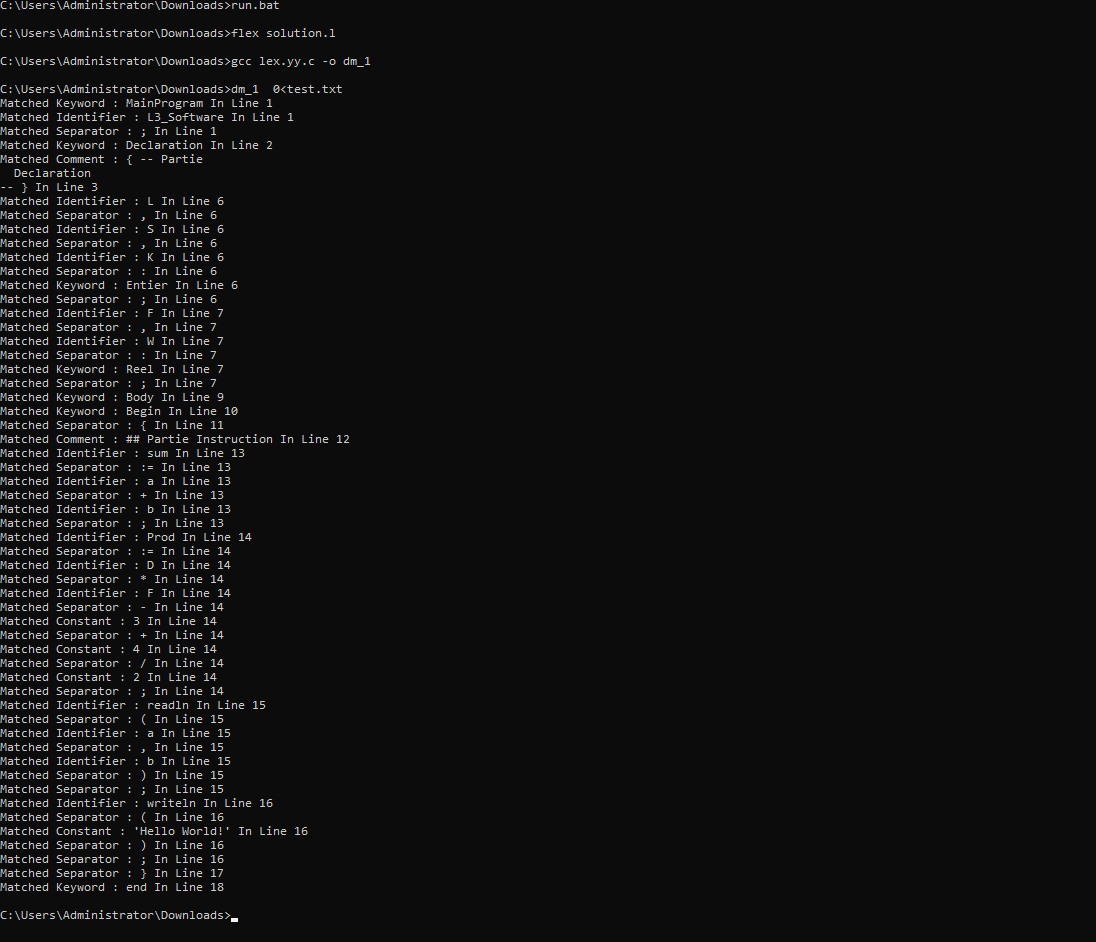
\includegraphics[width=\textwidth]{Parts/output.PNG}
\end{center}


\end{document}
